\documentclass{article}

\usepackage[utf8]{inputenc} % Required for inputting international characters
\usepackage[T1]{fontenc} % Output font encoding for international characters
\usepackage[backend=bibtex,style=alphabetic,natbib=true]{biblatex}
\addbibresource{references.bib}
\usepackage{amsmath, amssymb, amsfonts, amsthm, stmaryrd}
\usepackage{caption}
\usepackage{subcaption}
\usepackage{graphicx}
\usepackage{enumitem}
\usepackage{mathpartir}
\usepackage{bussproofs}
\usepackage{xparse}
\usepackage[usenames, dvipsnames]{xcolor}
\usepackage{lipsum}
\usepackage{xargs}
\usepackage{hyperref}
\usepackage{tikz-cd}
\usepackage{todonotes}
\usepackage{url}
\usepackage{xspace}
\usepackage{rotating}
\usepackage{quiver}
\usepackage[backend=bibtex,style=alphabetic,natbib=true]{biblatex}
\usepackage{minted}
\usepackage{newunicodechar}

\addbibresource{references.bib}
\usepackage{array}   % for \newcolumntype macro
\newcolumntype{C}{>{$}c<{$}} % math-mode version of "l" column type
\newcolumntype{L}{>{$}l<{$}} % math-mode version of "l" column type

% \usepackage{draftwatermark}
% \SetWatermarkText{Confidential}
% \SetWatermarkScale{4}
% \SetWatermarkColor[gray]{0.9}

\hypersetup{
  linktocpage,
  colorlinks,
  citecolor=BlueViolet,
  filecolor=red,
  linkcolor=Blue,
  urlcolor=BrickRed
}
\newcommand{\mpav}[1]{\textcolor{red}{\textsc{Marco}: #1}}
\newcommand{\proofcomment}[1]{\text{\{ #1 \}}}
\newenvironment{proofof}[1] {\begin{proof}[Proof of {#1}]}{\end{proof}}
\newcommand{\eqdef}{\stackrel{\mathrm{\Delta}}{=}}
\newcommand{\bnfeq}{\mathrel{::=}}
\newcommand{\defeq}{\triangleq}
\newcommand{\rul}[3]{\frac{#2}{#3}\;  {\textrulelabel{#1}}}
\newcommand{\den}[1]{\llbracket #1 \rrbracket}
\newcommand{\jud}[3]{#1 \vdash #2 : #3}
\newcommand{\bden}[1]{\llparenthesis#1 \rrparenthesis}
\newcommand{\bigslant}[2]{{\raisebox{.2em}{$#1$}\left/\raisebox{-.2em}{$#2$}\right.}}
\newcommand{\quotient}[2]{\bigslant{#1}{#2}}

\newcommand{\curry}{\Lambda}
\newcommand{\uncurry}{\begin{sideways}\begin{sideways}$\Lambda$\end{sideways}\end{sideways}}

\newcommand{\Bool}{\mathbb{B}}
\newcommand{\N}{\mathbb{N}}
\newcommand{\Nat}{\N}
\newcommand{\Sets}{\mathbf{Set}}
\newcommand{\blacklater}{\blacktriangleright}
\newcommand{\tot}{\mathcal{S}}
\newcommand{\PSh}{\ensuremath{\textbf{PSh}(\omega)}}

\newsavebox{\lbananabox}
\newcommand{\lbananamacro}{%
  
\begin{tikzpicture}[baseline=0.25em,xscale=0.005em,yscale=0.005em]
  \draw[solid, join=round] (2,0) to[out=140,in=-90] (0,3) to[out=90,in=-140] (2,6) -- (2.1,5.9)
              to[out=-120,in=90] (1.2,3) to[out=-90,in=120] (2.1,0.1) -- cycle;
\end{tikzpicture}
}
\savebox{\lbananabox}{\lbananamacro}
\newcommand{\lbanana}{\mathopen{\usebox{\lbananabox}\hspace{-0.6ex}}}


\newsavebox{\rbananabox}
\newcommand{\rbananamacro}{%
  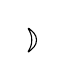
\begin{tikzpicture}[baseline=0.25em,xscale=-0.005em,yscale=0.005em]
  \draw[solid, join=round] (2,0) to[out=140,in=-90] (0,3) to[out=90,in=-140] (2,6) -- (2.1,5.9)
              to[out=-120,in=90] (1.2,3) to[out=-90,in=120] (2.1,0.1) -- cycle;
  \end{tikzpicture}
}
\savebox{\rbananabox}{\rbananamacro}
\newcommand{\rbanana}{\mathclose{\usebox{\rbananabox}}}


\newsavebox{\lbansbox}
\newcommand{\lbansmacro}{%
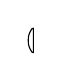
\begin{tikzpicture}[baseline=0.45ex,xscale=0.006em,yscale=0.012ex]%
% curvey bananas
%\draw[solid,join=round,fill=yellow] (2,0) to[out=140,in=-90] (0,3) to[out=90,in=-140] (2,6) -- (2.1,5.9) to[out=-120,in=90] (1.2,3) to[out=-90,in=120] (2.1,0.1) -- cycle;%
% fitted lenses
\draw[solid,join=round] (1.8,6) -- (1.5,5.9) to[out=-120, in=90] (0.7,3) to[out=-90, in=120] (1.5,0.1) -- (1.8,0) -- cycle;%
\end{tikzpicture}}
\savebox{\lbansbox}{\lbansmacro}
\newcommand{\lbans}{\mathopen{\usebox{\lbansbox}\mspace{1mu}}}

\newsavebox{\rbansbox}
\newcommand{\rbansmacro}{%
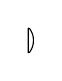
\begin{tikzpicture}[baseline=0.45ex,xscale=-0.006em,yscale=0.012ex]%
% curvey bananas
%\draw[solid,join=round,fill=yellow] (2,0) to[out=140,in=-90] (0,3) to[out=90,in=-140] (2,6) -- (2.1,5.9) to[out=-120,in=90] (1.2,3) to[out=-90,in=120] (2.1,0.1) -- cycle;%
% fitted lenses
\draw[solid,join=round] (1.8,6) -- (1.5,5.9) to[out=-120, in=90] (0.7,3) to[out=-90, in=120] (1.5,0.1) -- (1.8,0) -- cycle;%
\end{tikzpicture}}
\savebox{\rbansbox}{\rbansmacro}
\newcommand{\rbans}{\mathclose{\mspace{1mu}\usebox{\rbansbox}}}

\newsavebox{\llensbox}
\newcommand{\llensmacro}{%

\begin{tikzpicture}[baseline=0.45ex,xscale=0.006em,yscale=0.012ex]%
\draw[solid,join=round] (1.4,0) -- (0,0) -- (0,6) -- (1.4,6) -- (1.5,5.9) to[out=-120, in=90] (0.7,3) to[out=-90, in=120] (1.5,0.1) -- cycle;%
\end{tikzpicture}}
\savebox{\llensbox}{\llensmacro}
\newcommand{\llens}{\mathopen{\usebox{\llensbox}\mspace{1mu}}}

\newsavebox{\rlensbox}
\newcommand{\rlensmacro}{%
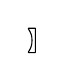
\begin{tikzpicture}[baseline=0.45ex,xscale=-0.006em,yscale=0.012ex]%
\draw[solid,join=round] (1.4,0) -- (0,0) -- (0,6) -- (1.4,6) -- (1.5,5.9) to[out=-120, in=90] (0.7,3) to[out=-90, in=120] (1.5,0.1) -- cycle;%
\end{tikzpicture}}
\savebox{\rlensbox}{\rlensmacro}
\newcommand{\rlens}{\mathclose{\mspace{1mu}\usebox{\rlensbox}}}

% filled versions
\newcommand{\Lbanana}{%
  \mathopen{\mspace{1mu}\tikz[baseline=0.25em,xscale=0.006em,yscale=0.006em]
  \fill (2,0) to[out=140,in=-90] (0,3) to[out=90,in=-140] (2,6) -- (2.1,5.9)
              to[out=-120,in=90] (1.2,3) to[out=-90,in=120] (2.1,0.1) -- cycle;\mspace{1mu}}}
\newcommand{\Rbanana}{%
  \mathclose{\mspace{1mu}\tikz[baseline=0.25em,xscale=-0.006em,yscale=0.006em]
  \fill (2,0) to[out=140,in=-90] (0,3) to[out=90,in=-140] (2,6) -- (2.1,5.9)
              to[out=-120,in=90] (1.2,3) to[out=-90,in=120] (2.1,0.1) -- cycle;}}
% % lens brackets (using TikZ)
% \newcommand{\llens}{%
%   \mathopen{\tikz[baseline=0.25em,xscale=0.006em,yscale=0.006em]
%   \draw[join=round] (1.4,0) -- (0,0) -- (0,6) -- (1.4,6) -- (1.5,5.9)
%         to[out=-120,in=90] (0.7,3) to[out=-90,in=120] (1.5,0.1) -- cycle;\mspace{1mu}}}
% \newcommand{\rlens}{%
%   \mathclose{\mspace{1mu}\tikz[baseline=0.25em,xscale=-0.006em,yscale=0.006em]
%   \draw[join=round] (1.4,0) -- (0,0) -- (0,6) -- (1.4,6) -- (1.5,5.9)
%         to[out=-120,in=90] (0.7,3) to[out=-90,in=120] (1.5,0.1) -- cycle;}}
% filled versions
\newcommand{\Llens}{%
  \mathopen{\tikz[baseline=0.25em,xscale=0.006em,yscale=0.006em]
  \fill (1.4,0) -- (0,0) -- (0,6) -- (1.4,6) -- (1.5,5.9)
        to[out=-120,in=90] (0.7,3) to[out=-90,in=120] (1.5,0.1) -- cycle;\mspace{1mu}}}
\newcommand{\Rlens}{%
  \mathclose{\mspace{1mu}\tikz[baseline=0.25em,xscale=-0.006em,yscale=0.006em]
  \fill (1.4,0) -- (0,0) -- (0,6) -- (1.4,6) -- (1.5,5.9)
        to[out=-120,in=90] (0.7,3) to[out=-90,in=120] (1.5,0.1) -- cycle;}}


\newcommand{\anamor}[1]{{\llens\, #1\, \rlens}}
\newcommand{\catamor}[1]{\lbans\, #1\, \rbans}
\newcommand{\cata}[1]{\lbans #1 \rbans}
\newcommand{\ana}[1]{\llens #1 \rlens}
\newcommand{\fold}[1]{\catamor{#1}}
\newcommand{\unfold}[1]{\anamor{#1}}
\newcommand{\comp}{\cdot}
\newcommand{\operator}[1]{\textsf{#1}}
\newcommand{\Alg}{\text{-Alg}}
\newcommand{\Free}{\text{Free\xspace}}

\newcommand{\CatC}{\mathcal{C}}
\newcommand{\CatD}{\mathcal{D}}
\newcommand{\CatE}{\mathcal{E}}
\newcommand{\CatI}{\mathcal{I}}

\newcommand{\Set}{\mathbf{Set}}
\newcommand{\iso}{\cong}
\newcommand{\ceiling}[1]{\lceil #1 \rceil}
\newcommand{\floor}[1]{\lfloor #1 \rfloor}

\newcommand{\pair}[2]{\langle #1, #2 \rangle}
\newcommand{\InIso}{\text{In}}

\newcommand{\haskell}[1]{\mintinline{haskell}{#1}}

\title{A Mechanised Library for Generic (Co)Programming}

\author{}

\begin{document}

\maketitle
\section{Introduction}
Recursive definitions cannot be proven well-defined automatically due to the
halting problem. Modern proof assistants like Coq or Agda provide a sound, but
incomplete algorithm which syntactically checks for termination or productivity.
For recursion, this is done by trying to (automatically) infer which argument in
the recursive call gets smaller with respects to the original input argument.
For productivity, the algorithm checks that the (co)recursive call appears
directly under a constructor to make sure that this function always produce at
least one element after each recursive step.

As mentioned, some functions, though well-defined, cannot be accepted by the
proof assistant. One example is the quicksort algorithm. This is given by the \haskell{partition} and \haskell{quicksort} function below (written in
Haskell code):
\begin{minted}{haskell}
partition :: [a] -> ([a], a, [a])
partition (x:xs) = (filter (x <=) xs, x, filter (x >) xs)

quicksort :: [a] -> [a]
quicksort [] = []
quicksort ls = let (xs, x, ys) = partition ls in
                        (quicksort xs) ++ [x] ++ (quicksort ys)
\end{minted}
While \haskell{quicksort} is a well-defined mathematical function it cannot be
accepted by a proof assistant.  The reason is that the \haskell{partition}
function \emph{destructuring} the input ``dives'' deeper in the input returning
two sublists with the head as a pivot.

A pen-and-paper technique would be to show that the \haskell{partition} is a
\emph{well-founded coalgebra} on the functor $(- \times A \times -)$ for a fixed
type $A$. Here the term ``well-founded'' refers to the fact that the infinite
iteration of this coalgebra will produce a \emph{finite} binary tree with nodes
in $A$.

More generally, this is an instance of a \emph{divide-and-conquer} algorithm.
Such algorithms are structured in three parts: first, the input is broken down
in smaller sub-problems by means of a well-founded coalgebra. Secondly, these
sub-problems are computed recursively and, finally, the results of the recursive
call are put together by a an algebra. This particular way of doing recursion
has been named in the functional programming literature as a
hylomorphism~\cite{MeijerFP91, HuIT96}.

Many years later Hinze et al.~\cite{HinzeWG15} showed that every recursive
program can be turned into an hylomorphism by means of the conjugate rule. The
essence of this result is that every complex recursion scheme can be explained
by its associated \emph{adjunction} which establishes a way of reducing the
proof obligation for the complex recursion scheme into the proof obligation for
a basic hylomorphism. This can be paraphrased by saying
\begin{center}
  ``\emph{every recursion scheme can be formalised as an hylomorphism}''
\end{center}

This result has given a much needed unifying view of recursion scheme which
helped understanding their nature and also in providing a unified way of
reasoning about recursive programs by means of fusion laws.

All in all, the functional programming way of dealing with recursion is to just
allow all types of recursion and then restricting ourselves to only the
recursion schemes provided by the given libraries. This gives a way of ``fast
and loose reasoning''~\cite{DanielssonHJG06} which works provided that the user
is somewhat aware of the perils of feeding this libraries with potentially
non-terminating programs.

The type theoretical approach instead is to reject all definitions which cannot
be proven well-defined. It is safer, but incomplete.

With this work we intend to begin a study of the applications of recursion
schemes that goes beyond functional programming, that is to dependent type
theories such as a the ones employed in proof assistants like Agda or Coq where
non-termination is outright rejected.

This has been a long-standing challenge to come up with a sound algorithm which
rejects all programs that do not terminate (soundness) and accepts as many
well-defined programs as possible (completeness). Our aim is to provide an
additional tool to the every-day programmer to be able to extend the range of
recursive programs we can write.

One of the challenges here is to be able to keep the theory of recursions
schemes as general as possible while maintaining its practical usefulness. In
order to do this, we have to make some design choices which differ a bit from
the general theory.  For instance, formalising the conjugate rule would require
us to mechanise a non-trivial fragment of category theory inside the prover's
logic.  Secondly, the general conjugate rule is a statement of correspondence of
arrows rather than a proof that these programs actually exists. In functional
programming languages like for instance Haskell this is not a problem, since
every functor is strong and has a fixed-point.  On the other hand, in a type
theory we have to restrict to those so-called polynomial functors. In this work
we do not make use of these assumptions. By restricting ourselves to polynomial
functors given in terms of containers~\cite{AbbottAG05} we are able to prove the
recursion schemes within the proof assistant and at the same time to maintain a
certain level of data abstraction.

First we prove that the hylo equation has a unique solution
\[
  x = a \comp F(x) \comp c
\]
for every recursive coalgebra $c$ for a polynomial $F$. Then we prove each
recursion scheme by reducing it to a hylo. The following recursion schemes can
all be proven by reducing them to an hylo: folds, mutual recursive functions,
recursion schemes from comonads and their respective coinductive dual.

The contributions we make in this paper are as follows:
\begin{itemize}
  \item We provide a framework for \emph{generic programming} with recursion
schemes in Coq
  \item We formalise algorithms for divide and conquer, dynamic programming and
mutual recursion
  \item We validated optimisations in Coq and extract the resulting code to
OCaml.
\end{itemize}

\section{Background on Adjoint Folds}
Say that we want to prove that the two functions below are well-defined

\begin{tabular}{LL}
  \operator{even} : \Nat \to \Bool                  &  \operator{odd} : \Nat \to \Bool\\
  \operator{even} (0) = \top                        &  \operator{odd}(0) = \bot\\
  \operator{even} (n+1) = \neg \operator{odd}(n)    &  \operator{odd}(n+1) = \neg (\operator{even}(n))
\end{tabular}

One option is to prove that the following function (given by a catamorphism) is
equivalent to the above
\begin{align*}
  & \operator{even-odd} : \Nat \to \Bool \times \Bool\\
  & \operator{even-odd} (0) = (\top, \bot)\\
  & \operator{even-odd} (n+1) = \operator{let } (x,y) \leftarrow \operator{even-odd}(n) \operator{ in } (\neg x, \neg y)
\end{align*}
This function is clearly a catarmorphism:
\begin{align*}
  & \operator{even-odd} : \Nat \to \Bool \times \Bool\\
  & \operator{even-odd} = \cata{a} \operator{ where }\\
  & \qquad \qquad a : 1 + (\Bool \times \Bool)\\
  & \qquad \qquad a (\operator{nil}) = (\top, \bot)\\
  & \qquad \qquad a (\operator{x,y}) = (\neg x, \neg y)
\end{align*}
where $\cata{\cdot}$ takes a $(1+-)$ algebra on $\Bool \times \Bool$ and returns
the associated recursive function.

Now we recover the original two functions by setting
$\operator{even}' \eqdef \pi_{1} \comp \operator{even-odd}$
$\operator{odd}' \eqdef \pi_{2} \comp \operator{even-odd}$. The proof that these
two pairs of functions are the same is an easy induction over the natural
numbers.

This is an instance of a more general phenonema whose argumet uses category
theory.

\section{Adjoint Folds}
In order to transform $\operator{even-odd}$ into two functions $\operator{even}$
and $\operator{odd}$ we are going to use something called an ``adjunction''.  In
particular, we have two functors. The diagonal functor
$\Delta : \CatC \to \CatC \times \CatC$ defined as $\Delta X = (X,X)$ and the
product functor $\times : \CatC \times \CatC$. These two functors form an
adjunction:
\[\begin{tikzcd}
	{\CatC \times \CatC} & \CatC
	\arrow[""{name=0, anchor=center, inner sep=0}, "\Delta"', shift right=2, from=1-2, to=1-1]
	\arrow[""{name=1, anchor=center, inner sep=0}, "\times"', shift right=2, from=1-1, to=1-2]
	\arrow["\dashv"{anchor=center, rotate=-90}, draw=none, from=0, to=1]
    \arrow["D"', loop, distance=2em, in=35, out=325, from=1-2, to=1-2]
    \arrow["\Delta\circ D\circ \times "', loop, distance=2em, in=215, out=145, from=1-1, to=1-1]
\end{tikzcd}
\]
More formally, this means there is a one-to-one correspondence of maps, i.e.
every map $(A,A) \to (B_{1}, B_{2})$ corresponds univocally to a map of type
$A \to B_{1} \times B_{2}$. In the isomorphism below we use $\ceiling{\cdot}$
and $\floor{\cdot}$ to denote the maps witnessing the isomorphism called
respectively the right and left transpose of the adjunction:
\[
  \floor{\cdot} : \CatC \times \CatC ((A, A) , (B_{1}, B_{2}) \iso \CatC (A , B_{1} \times B_{2}): \ceiling{\cdot}
\]
the right transponse $\ceiling{\cdot}$ of the adjunction can be
defined using the projections:
\[
  \ceiling{g} = (\pi_{1} \cdot g,\pi_{2}\cdot g)
\]
and the floor can be defined as using the pair into the product:
\[
  \floor{f}(a) = \pair{f(a)}{f(a)}
\]

We can instantiate further the iso by setting $A = \Nat$, $B_{1} = \Bool$ and
$B_{2} = \Bool$.
\[
  \floor{\cdot}: \CatC \times \CatC ((\Nat, \Nat) , (\Bool, \Bool) \iso \CatC (\Nat , \Bool \times \Bool) : \ceiling{\cdot}
\]
% At this point we are pretty much done as we can instantiate the diagrams
% (\ref{eq:canonical-adjoint-fold}) where $D X = 1 + X$
% \[
%   \begin{tikzcd}
% 	{(1 + \Nat, 1 + \Nat)} && (1 + \Bool \times \Bool, 1 + \Bool \times \Bool) & { 1 + \Nat} & 1 + (\Bool \times \Bool) \\
% 	{(\Nat, \Nat)} && (\Bool, \Bool) & {\Nat} & \Bool \times \Bool
% 	\arrow["{\cata{a}}"', from=2-4, to=2-5]
% 	\arrow[""{name=0, anchor=center, inner sep=0}, "{\InIso}"', from=1-4, to=2-4]
% 	\arrow["{1 + \cata{a}}", from=1-4, to=1-5]
% 	\arrow["a", from=1-5, to=2-5]
% 	\arrow["{\ceiling{\cata{a}}}"', from=2-1, to=2-3]
% 	\arrow["{(1 +  \InIso,1 +  \InIso)}"', from=1-1, to=2-1]
% 	\arrow["{(1 + \cata{a}, 1 + \cata{a})}", from=1-1, to=1-3]
% 	\arrow[""{name=1, anchor=center, inner sep=0}, "\ceiling{a}", from=1-3, to=2-3]
% 	\arrow[shorten <=35pt, shorten >=35pt, Rightarrow, 2tail reversed, from=1, to=0]
%   \end{tikzcd}
% \]
% Now we define $a$ to be the following $D$ algebra:
% \begin{align*}
%   & a : 1 + \Bool \times \Bool \to \Bool\\
%   & a (\operator{nil}) = (\top, \bot)\\
%   & a (b_{1}, b_{2}) = (\neg b_{1}, \neg b_{2})
% \end{align*}

We already seen that the catamorphism over the algebra $a$ equals
$\operator{even-odd}$. By using the right transpose we can derive the pair of
original functions $(\operator{even}, \operator{odd})$:
\[
  \ceiling{\operator{even-odd}} = (\pi_{1}\cdot \operator{even-odd}, \pi_{2}\cdot \operator{even-odd})
\]
To show this pair of functions are the same as the original ones we appeal to
uniqueness of catamorphisms. Recall that catamorphisms for a generic $F$ algebra
$a$ are the unique maps such that
\[
  \cata{a} = a \comp F(\cata{a})\comp \InIso^{\circ}
\]
This is represented on the right hand side of the following diagrams:
\[
  \begin{tikzcd}
	{(1 + \Nat, 1 + \Nat)} && (1 + \Bool^{2}, 1 + \Bool^{2}) & {1 + \Nat} & 1 + \Bool^{2} \\
	{(\Nat, \Nat)} && (\Bool, \Bool) & {\Nat} & \Bool^{2}
	\arrow["{\operator{eo}}"', dotted,  from=2-4, to=2-5]
	\arrow[""{name=0, anchor=center, inner sep=0}, "{\InIso}"', from=1-4, to=2-4]
	\arrow["{1 + \operator{eo}}", dotted, from=1-4, to=1-5]
	\arrow["a", from=1-5, to=2-5]
	\arrow["{\ceiling{\operator{eo}}}"', from=2-1, to=2-3]
	\arrow["{(1 +  \InIso,1 +  \InIso)}"', from=1-1, to=2-1]
	\arrow["{(1 + \operator{eo}, 1 + \operator{eo})}", from=1-1, to=1-3]
	\arrow[""{name=1, anchor=center, inner sep=0}, "\ceiling{a}", from=1-3, to=2-3]
	\arrow[shorten <=20pt, shorten >=20pt, Rightarrow, 2tail reversed, from=1, to=0]
  \end{tikzcd}
\]
The double implication in the middle of these two diagrams states that the
catamorphism on the right is in one-to-one correspondences with the right
transpose of $\operator{eo}$ satisfying the right-hand side diagram. Notice the
right-hand side is exactly the definition of the pair of functions
$\operator{even}$ and $\operator{odd}$ and the diagram states these correspond
to $\operator{even-odd}$ given by a catamorphism on the left. Since this latter
is the unique catamorphism the one on the right is also unique such that it
makes the right-hand side diagram commute.

\subsection{The General Case}

\[\begin{tikzcd}
	{\CatC} & \CatD
	\arrow[""{name=0, anchor=center, inner sep=0}, "L"', shift right=2, from=1-2, to=1-1]
	\arrow[""{name=1, anchor=center, inner sep=0}, "R"', shift right=2, from=1-1, to=1-2]
	\arrow["\dashv"{anchor=center, rotate=-90}, draw=none, from=0, to=1]
    \arrow["D"', loop, distance=2em, in=35, out=325, from=1-2, to=1-2]
    \arrow["LDR"', loop, distance=2em, in=215, out=145, from=1-1, to=1-1]
\end{tikzcd}
\]

The following is a natural isomorphism arising from the adjunction $L \dashv R$.
\begin{equation}
  \label{eq:adjoint-iso}
  \floor{\cdot} : \CatC(LA, B) \iso \CatD (A, RB) : \ceiling{\cdot}
\end{equation}
Some properties of adjunctions are worth recalling.  The unit and counit of the
adjunction can be defined from the above isomorphism as follows:
\[
  \eta_{A} = \floor{id_{LA}} \qquad \epsilon_{B}  = \ceiling{id_{RB}}
\]
Conversely, the isomorphism can be defined in terms of the two functors $L$ and
$R$ and the units of the adjunction:
\begin{align*}
  & \floor{f : LA \to B} = A \xrightarrow{\eta_{A}} RLA \xrightarrow{R(f)} RB\\
  & \ceiling{g : A \to RB} = LA \xrightarrow{L(g)} LRB \xrightarrow{\epsilon_{B}} B
\end{align*}
These definitions are going to be useful later to understand the definitions of
the recursion schemes we are going to prove correct.

As a result, the following two diagrams (recursion schemes) are equivalent. The
on the right hand side is a \emph{catamorphism} taking a $D$ algebra on $RB$ and
construting an inductive function over the data type $\mu D$. The one on the
left hand side is the derived recursion scheme where the data type has been
wrapped up in $L$. The transformation is done by just applying the isomorphism
(\ref{eq:adjoint-iso}) given by the adjunction.

\begin{equation}
  \label{eq:canonical-adjoint-fold}
  \begin{tikzcd}
	{LD\mu D} & LDRB && {D\mu D} & DRB \\
	{L\mu D} & B & {} & {\mu D} & RB
	\arrow["{\cata{a}}"', from=2-4, to=2-5]
	\arrow[""{name=0, anchor=center, inner sep=0}, "{\InIso}"', from=1-4, to=2-4]
	\arrow["{D(\cata{a})}", from=1-4, to=1-5]
	\arrow["{\floor{a}}", from=1-5, to=2-5]
	\arrow["{\ceiling{\cata{a}}}"', from=2-1, to=2-2]
	\arrow["{L(\InIso)}"', from=1-1, to=2-1]
	\arrow["{LD(\cata{a})}", from=1-1, to=1-2]
	\arrow[""{name=1, anchor=center, inner sep=0}, "a", from=1-2, to=2-2]
	\arrow[shorten <=28pt, shorten >=28pt, Rightarrow, 2tail reversed, from=1, to=0]
  \end{tikzcd}
\end{equation}

In the following section we instantiate the adjoint fold with some instances
taken from the literature.

\section{Related Work}

\begin{itemize}
  \item McBride devised a generalisation of Bove and Capretta's general
recursive function monad~\cite{McBride15, BoveC01}
  \item Guarded recursion for productive definitions and general recursion
~\cite{AtkeyM13, PaviottiMB15}
  \item PACO library~\cite{HurNDV13}
  \item Sized Types \cite{AbelPTS13, AbelP16}
\end{itemize}

\printbibliography[heading=bibintoc]

\end{document}

%%% Local Variables:
%%% TeX-command-extra-options: "-shell-escape"
%%% End:
